%
% Theory
%

% !TEX root = ../../main.tex

\chapter{Grundlagen}

  \section{Natürliche vs.\ artifizielle Evolution}

    Natürliche Evolution hat kein vordefiniertes Ziel und ist ein sogenannter ``open-ended'' Anpassungsprozess.
    Unter einem ``open-ended'' Anpassungsprozess in der natürlichen Evolution
    versteht man die Anpassung an die natürliche Umgebung.
    Da sich die natürliche Umgebung stetig ändert, ist der Prozess immer im Gange und endet nie.
    Artifizielle Evolution jedoch ist ein Optimierungsprozess,
    welcher versucht Lösungen zu vordefinierten Problemen zu finden~\cite[S.1]{book:bioInspired}.

  \section{Artifizielle Evolution}

    \subsection{Individuum\label{sub:individual}}

      Als Individuum wird die zu evolvierende künstliche Kreatur bezeichnet.
      Ein Individuum hat einen zugehörigen Genotyp~(\vref{sub:genotyp}) und einen Phänotyp~(\vref{sub:introPhenotyp}).

    \subsection{Genotyp\label{sub:genotyp}}

      Das genetische Material eines Individuums wird als Genotyp bezeichnet~\cite[S.5]{book:bioInspired}.
      Es beinhaltet alle wichtigen Informationen zur Reproduktion des Individuums.

    \subsection{Genom\label{sub:genom}}

      Das Genom ist eine Repräsentation des Genotyps.
      Es beinhaltet nur Werte, jedoch keine Information was diese bedeuten.
      Erst durch den Geno- und Phänotyp werden den Werten einen Sinn gegeben.

    \subsection{Phänotyp\label{sub:introPhenotyp}}

      Der Phänotyp ist das Erscheinungsbild eines Individuums.
      Er wird aus dem Genotyp und externen Faktoren gebildet.
      \\
      Ein Individuum welches durch den Genotyp beschrieben wird, nimmt durch den Phänotyp eine sichtbare Form an.
      Wenn der Genotyp die Länge und Breite eines Rechtecks beschreibt,
      so ist das grafisch gezeichnete Rechteck auf dem Monitor der Phänotyp~(\vref{fig:genoPheno}).

      \begin{figure}[H]
        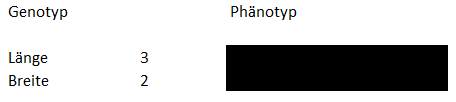
\includegraphics[scale=1,center]{graphics/genotyp_phenotyp}
        \caption{Genotyp und Phänotyp\label{fig:genoPheno}}
      \end{figure}

    \subsection{Genetische Repräsentation}

      Der erste Schritt bei der Definition eines evolutionären Algorithmus ist die Auswahl der genetischen Repräsentation.
      Nicht alle Arten von evolutionären Algorithmen harmonieren mit jeder Repräsentation.
      Die genetische Repräsentation beschreibt die Elemente eines Genoms und
      wie diese auf einen Phänotyp abgebildet werden~\cite[S.16]{book:bioInspired}.

      \subsubsection{Diskrete Repräsentation\label{subsub:GeneticRepresentationDiscrete}}

        Bei der diskreten Repräsentation kann das Genom als binären String dargestellt [0111110] werden.
        Dieser binäre String kann anschliessend in einen Phänotyp übersetzt werden.
        Zum Beispiel kann eine Bitsequenz, direkt zu einer Zahl als Phänotyp übersetzt werden [0011] -> 3.

        \medskip

        Eine diskrete Repräsentation kann ebenfalls eine Folge von beliebigen Zeichen annehmen [ABCDEF].
        D. Floreano und C. Mattiussi~\cite[S.18]{book:bioInspired} zeigen dies anhand des ``Travelling Sales Man Problems'':
        Jeder Buchstabe in der Sequenz repräsentiert dabei einen Ort,
        welchen es zu besuchen gilt~(\vref{fig:travelling})~\cite[S.18]{book:bioInspired}.

        \begin{figure}[H]
          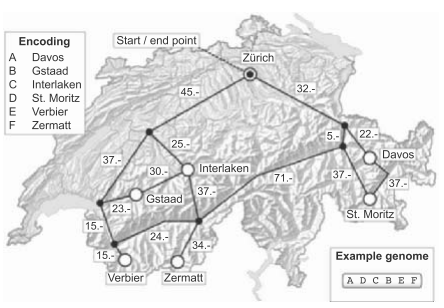
\includegraphics[scale=0.9,center]{graphics/discret_representation}
          \caption[\protect\bibentry{book:bioInspired}, S.18]{Beispiel Diskrete Repräsentation\label{fig:travelling}}
        \end{figure}

      \subsubsection{Reale-Werte-Repräsentation\label{subsub:GeneticRepresentationReal}}

        Weiter kann die Reale-Werte-Repräsentation gewählt werden.
        Das Genom~(\vref{fig:real_value_representation}) wird hierbei durch reelle Zahlen repräsentiert.
        Beispielsweise kann die optimale Position eines Zimmers (beste Flächennutzung) in einem Haus
        durch reale Zahlen dargestellt werden.

        \begin{figure}[H]
          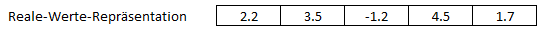
\includegraphics[scale=1,center]{graphics/real_value_representation}
          \caption{Beispiel Reale-Werte-Repräsentation\label{fig:real_value_representation}}
        \end{figure}

      \subsubsection{Baum-Repräsentationen\label{subsub:GeneticRepresentationTree}}

        Das zu evolvierende Objekt kann durch einen Baum dargestellt werden.
        \\
        Baum-Repräsentationen (\vref{fig:baum}) werden eingesetzt
        um hierarchische Strukturen mit Verzweigungen und Bedingungen zu beschreiben~\cite[S.19]{book:bioInspired}.
        Baumstrukturen haben den Vorteil, dass sie sehr gut rekursiv durchlaufen werden können.
        Viele Probleme aus der Informatik lassen sich einfacher rekursiv als iterativ lösen.

        \begin{figure}[H]
          \Tree[.* [.+ [.2 ] [.7 ] ].+ [.- [.5 ] [.1 ] ] ].*
          \caption{Darstellung einer Rechnung als Baum\label{fig:baum}}
        \end{figure}

    \subsection{Initiale Population}

      Die Grösse der zu evolvierenden Population kann selber bestimmt werden.
      Jedoch muss beachtet werden, dass eine grössere Population mehr Rechenaufwand bedeutet.
      Auch die Eigenschaften des Suchraums dürfen dabei nicht ignoriert werden.
      \\
      Wichtig bei der Erstellung einer initialen Population ist,
      möglichst diverse~(\vref{sub:diversity}) Individuen zu generieren,
      damit nicht wertvolle Lösungen verspielt werden.

    \subsection{Fitnessfunktion}

      Mit Hilfe der Fitnessfunktion lassen sich Individuen beurteilen,
      wie gut geeignet ihre Gene sind, um die Problemstellung zu bewältigen.
      In der natürlichen Evolution ist die Fitness des Tieres, wie viele Nachkommen es erzeugen kann.
      \\
      In der technischen Welt jedoch muss der Anwender sie jeweils selbst definieren und
      anhand der Problemstellung anpassen. Oft ist die Evaluation der Fitness-Funktion
      die rechenintensivste Teilaufgabe eines evolutionären Algorithmus~\cite[S.22]{book:bioInspired}.

    \subsection{Diversität\label{sub:diversity}}

      Die Diversität einer Population von Individuen beschreibt, wie verschieden die Individuen zueinander sind.
      Durch diese Kennzahl alleine lässt sich jedoch noch keine Aussage über die Diversität treffen.
      Erst wenn mehrere Generationen von Populationen vorhanden sind,
      kann diese Kennzahl benutzt werden um die Diversität zu beurteilen.
      Eine nummerisch grössere Zahl deutet darauf hin, dass die Individuen divers sind.

    \subsection{Selektionsoperation}

      Eine Selektionsoperation hilft die geeignetsten Individuen einer Generation zu selektieren.
      Die Selektierten bilden die Basis für die nächste Generation.
      Eine grosse Herausforderung beim Selektieren ist die Erhaltung der Diversität.

      \subsubsection{Selektionsdruck\label{subsub:SelectionPressure}}

        Als Selektionsdruck wird der Prozentsatz der Individuen der aktuellen Generation bezeichnet,
        welche man verwendet um Nachkommen zu erzeugen.
        Ein hoher Selektionsdruck bedeutet,
        dass nur wenige Individuen zur Reproduktion selektiert werden~\cite[S.23]{book:bioInspired}.

      \subsubsection{Proportionale Selektion}

        Bei der proportionalen Selektion wird die Reproduktionsrate proportional zur Fitness gewählt.
        D. Floreano und C. Mattiussi~\cite[S.23]{book:bioInspired} beschreiben die proportionale Selektion als Rouletterad,
        in dem jedes Individuum ein Stück des Rouletterads für sich beanspruchen~(\vref{fig:rouletteWheel}).
        Das Stück welches sie beanspruchen, ist so gross,
        wie ihre Fitness im Vergleich zu der Fitness ihrer Konkurrenten.
        \\
        Das Individuum mit der grössten Fitness wird auch das grösste Stück des Rouletterads für sich beanspruchen und hat somit die grösste Wahrscheinlichkeit, Nachkommen zu erzeugen.
        Wenn die Population \(N\) Individuen gross ist, wird das Rad \(N\) mal gedreht um die Nachkommen zu bestimmen.

        \medskip

        Proportionale Selektion funktioniert schlecht,
        wenn alle Individuen sehr ähnliche Fitnesswerte aufweisen oder es nur wenige/einen Ausreisser gibt.
        Denn dann haben alle Individuen die gleiche Chance selektiert zu werden.

        \begin{figure}[H]
          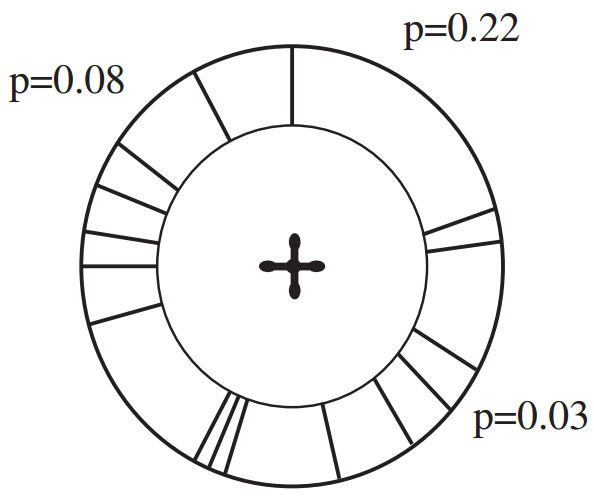
\includegraphics[scale=0.4,center]{graphics/roulettewheel}
          \caption[\protect\bibentry{book:bioInspired}, S.24]{Rouletterad der proportionalen Selektion\label{fig:rouletteWheel}}
        \end{figure}

      \subsubsection{Rangselektion}

        Es wird zuerst eine Rangliste nach Fitness erstellt und dann werden die Reproduktionswahrscheinlichkeiten proportional zum Rang zugeordnet.
        Anstatt das Rouletterad~(\vref{fig:rouletteWheel}) nach Fitness der Individuen zu unterteilen,
        wird es anhand des Ranges unterteilt.
        Diese Selektionsstrategie hat den Vorteil gegenüber der proportionalen Selektion,
        dass die Fitness der Individuen ähnlich sein darf,
        jedoch wird mit hoher Wahrscheinlichkeit das Bessere selektiert werden.

      \subsubsection{Gekürzte Rangselektion}

        Es wird eine Rangliste für die Individuen der Population erstellt.
        Anstatt alle Individuen zu berücksichtigen, werden nur die besten der Rangliste selektiert und diese produzieren Nachkommen (\vref{fig:truncated_rank_based_selection}).

        \begin{figure}[H]
          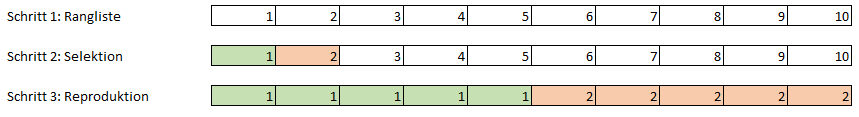
\includegraphics[width=\textwidth,center]{graphics/truncated_rank_based_selection}
          \caption{Schritte einer gekürzten Rangselektion\label{fig:truncated_rank_based_selection}}
        \end{figure}

      \subsubsection{Turnierselektion\label{subsub:Turnier}}

        Es werden \(k\) zufällig ausgewählte Individuen selektiert,
        diese Individuen tragen untereinander ein Turnier (\vref{fig:tournament_based}) aus.
        Das Turnier gewinnt jenes Individuum, welches den höchsten Fitnesswert aufweist.
        Dies wird solange wiederholt, bis so viele Nachkommen vorhanden sind wie in der vorherigen Generation.
        \\
        Ein grosser Vorteil von Turnierselektion ist die gute Balance zwischen
        Selektionsdruck und genetischer Diversität,
        da alle Individuen in der Population die gleiche Wahrscheinlichkeit haben, für das Turnier selektiert zu werden.
        Somit können auch Individuen mit niedrigem Fitnesswert ein Turnier gewinnen.

        \begin{figure}[H]
          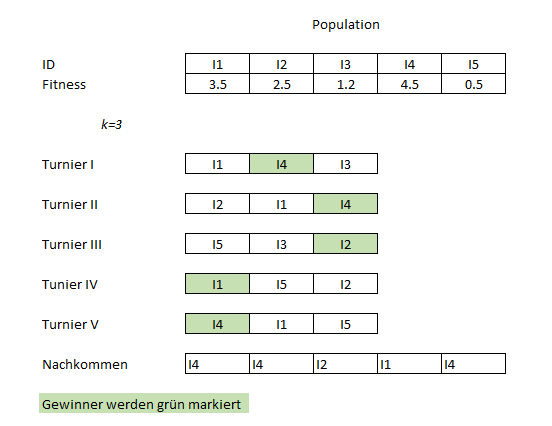
\includegraphics[scale=1,center]{graphics/tournament_based}
          \caption{Turnierselektion\label{fig:tournament_based}}
        \end{figure}

    \subsection{Rekombinationsfunktion}

      Bei der Rekombination werden jeweils zwei Individuen selektiert und
      deren Gen-Paare neu kombiniert (untereinander vertauscht).
      Die~\vref{fig:crossOver} veranschaulicht diesen Prozess.
      \\
      Nicht bei jedem Typ von evolutionären Algorithmen~(\vref{sub:artenEvAlgos}) und
      jeder Problemstellung ist Rekombination sinnvoll.
      Als Beispiel kann ein Haus mit Fenstern und Türen genommen werden.
      Dabei führt die Rekombination der Gene von Türen mit denen der Fenster zu keinen verwendbaren Resultaten.

      \begin{figure}[H]
        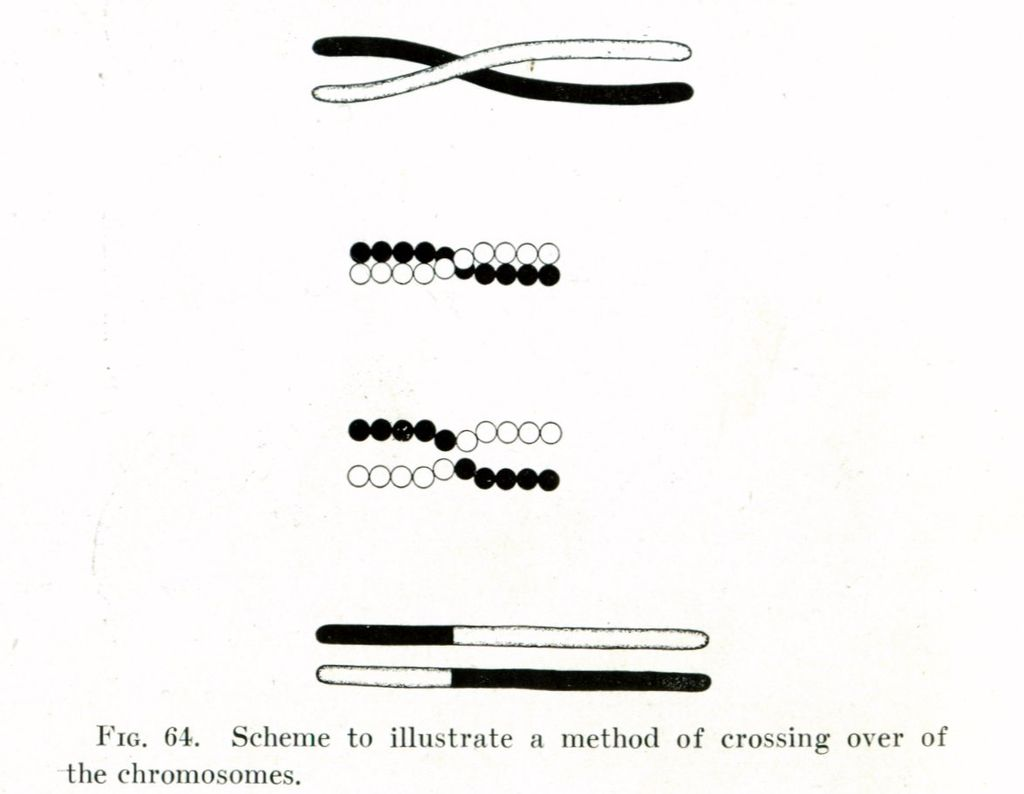
\includegraphics[scale=0.3,center]{graphics/morgan_crossover}
        \caption[\protect\bibentry{WikipediaEN:crossOver}]{Illustration des Crossover\label{fig:crossOver}}
      \end{figure}

      \subsubsection{One-Point-Crossover}

        Es wird ein zufälliger Cross-Over-Punkt bestimmt, an dem die Gene des Paares vertauscht werden (a)~\vref{fig:crossTypes}.
        Anwendbar ist diese Strategie bei Diskret- und Reale-Werte-Repräsentationen.

      \subsubsection{Multi-Point-Crossover}

        Dieser Ansatz funktioniert ähnliche wie One-Point-Crossover.
        Statt nur an einem Punkt, werden mehrere Punkte definiert an denen die Gene ausgetauscht werden.

      \subsubsection{Uniform-Crossover}

        Die Gene werden an \(n\) zufälligen Stellen vertauscht ( b)~\vref{fig:crossTypes}).

      \subsubsection{Arithmetic-Crossover}

        Der Durschnitt von den Genen an \(n\) zufälligen Positionen wird gebildet.
        Aus diesem Durchschnitt wird dann ein Nachkomme erzeugt ( c)~\vref{fig:crossTypes}).
        Da arithmetische Operationen nur auf Zahlen anwendbar sind,
        kann diese Art des Crossovers nur bei Reale-Werte-Repräsentationen verwendet werden.

      \subsubsection{Sequenzen}

        Bei Sequenzen muss die Regel eingehalten werden, dass alle Einträge nur einmal vorkommen dürfen.
        Es wird ein Multi-Point-Crossover durchgeführt unter Einhaltung der oben genannten Regel ( d)~\vref{fig:crossTypes}).

      \subsubsection{Bäume}

        Bei Bäumen wird ein zufälliger Teil eines Baumes,
        mit einem anderen zufälligen Teilbaum eines fremden Individuums vertauscht ( e)~\vref{fig:crossTypes}).

        \begin{figure}[H]
          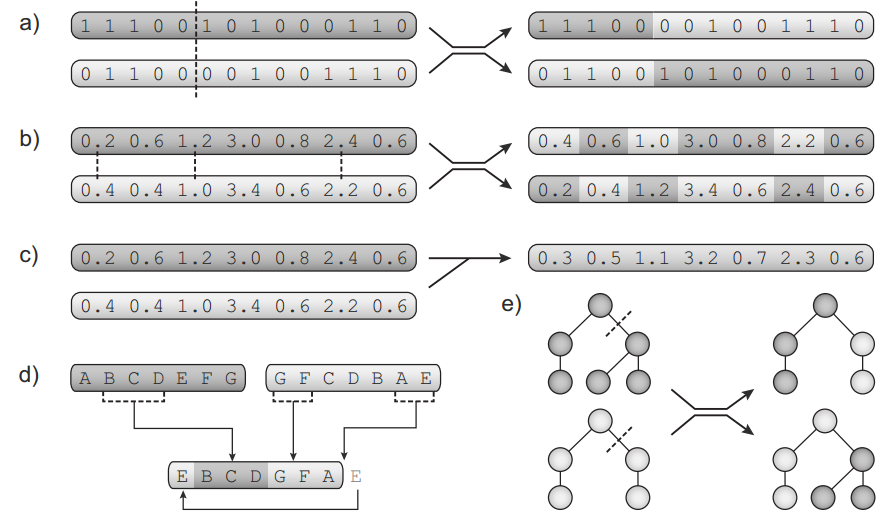
\includegraphics[width=\textwidth,center]{graphics/crossover_types}
          \caption[\protect\bibentry{book:bioInspired}, S.27]{Typen von Crossovers\label{fig:crossTypes}}
        \end{figure}

    \subsection{Mutationsfunktion~\label{sub:mutFunction}}

      Mutationen operieren auf dem Genotyp des Individuums.
      Die Positionen eines Genoms werden mit einer bestimmten Wahrscheinlichkeit \(p_{m}\) mutiert.
      \\
      Es ist jedoch Vorsicht geboten, da gewisse Lösungen durch Mutationen verloren gehen können~\cite{Sampson1976}.
      Wenn zu viel mutiert wird, kann die Selektion und Evolution der Individuen nicht stattfinden.
      Es wird dann eher eine Zufallssusche durchgeführt als eine richtige Evolution.
      Darum sollten Mutationswahrscheinlichkeiten klein gewählt werden.

      \subsubsection{Binäre Repräsentationen}

        Wenn die Repräsentation aus binären Werten besteht, werden die Bits invertiert (oder bestimmte Segmente).
        Invertieren bedeutet, dass aus einem 0 eine 1 wird und umgekehrt (\vref{fig:MutationBinaryFlip}).

        \begin{figure}[H]
          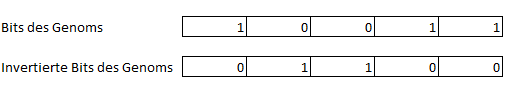
\includegraphics[scale=1,center]{graphics/mutation_binary_flip}
          \caption{Invertieren der Bits\label{fig:MutationBinaryFlip}}
        \end{figure}

      \subsubsection{Reale-Werte-Repräsentationen}

        Bei Realen-Werte-Repräsentation wird jeweils zu einem bestehenden Wert ein nummerischer Wert addiert.
        Der Wert sollte zufällig berechnet werden.
        Die Zufallsfunktion, welche dafür verwendet wird, sollte normalverteilt sein.
        Zudem sollte die Mutation innerhalb eines Wertebereichs stattfinden (\vref{fig:MutationRealValue}).

        \begin{figure}[H]
          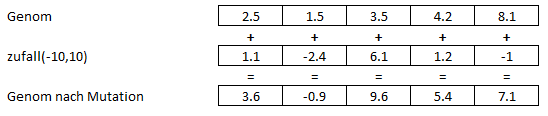
\includegraphics[scale=1,center]{graphics/mutation_real_value}
          \caption{Mutation von Reale-Werte-Repräsentationen\label{fig:MutationRealValue}}
        \end{figure}

      \subsubsection{Sequenzen}

        Zufällig ausgewählte Positionen der Sequenz werden miteinander vertauscht (\vref{fig:MutationSequences}).

        \begin{figure}[H]
            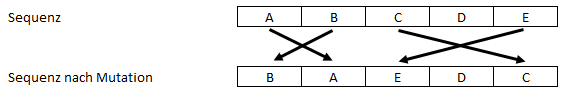
\includegraphics[scale=1,center]{graphics/mutation_sequences}
            \caption{Mutation von Reale-Werte-Repräsentationen\label{fig:MutationSequences}}
        \end{figure}

      \subsubsection{Baum}

        Bei Bäumen werden Teilabschnitte mutiert, wie in \vref{fig:MutationTree} erkennbar ist.

        \begin{figure}[H]
            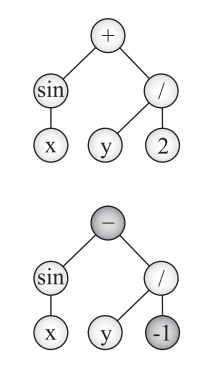
\includegraphics[scale=0.8,center]{graphics/mutation_tree}
            \caption[\protect\bibentry{book:bioInspired}, S.29]{Mutation von Bäumen\label{fig:MutationTree}}
        \end{figure}

    \subsection{Arten von evolutionären Algorithmen\label{sub:artenEvAlgos}}

      Es gibt verschiedene Typen von evolutionären Algorithmen, welche sich hauptsächlich in der Wahl ihrer
      genetischen Repräsentation und Operationen unterscheiden~\cite{book:introEvComp}.
      \\
      Die Auswahl des evolutionären Algorithmus hängt von den Eigenschaften der Problemstellung ab.
      Es gibt keinen Algorithmus der alle Probleme optimal lösen kann~\cite{book:genAlgoDataStructsEvProg}.
      Die am häufigsten verbreiteten Algorithmen sind: genetische Algorithmen~(\vref{item:genAlgo}),
      genetische Programmierung~(\vref{item:genProg}), evolutionäre Programmierung~(\vref{item:evProg})
      und evolutionäre Strategien~(\vref{item:evStrat}).

      \subsubsection{Genetische Algorithmen\label{item:genAlgo}}

        Die Genetischen Algorithmen~\cite{book:adapNaturalArtSys} arbeiten mit binären genetischen Repräsentationen.
        Es wird rekombiniert und selten mutiert~\cite[S.128]{book:evAlgo}.
        Die Mutationen werden, falls eingesetzt,
        nur mit einer sehr kleinen Wahrscheinlichkeit durchgeführt~\cite[S.128]{book:evAlgo}.

      \subsubsection{Genetische Programmierung\label{item:genProg}}

        Bei der genetischen Programmierung~\cite{book:genProg} werden Bäume als Repräsentation des Genoms eingesetzt.
        Wie bei den genetischen Algorithmen wird Rekombination eingesetzt.
        Als Nebenoperator kann Mutation eingesetzt werden~\cite[S.147]{book:evAlgo}.

      \subsubsection{Evolutionäre Programmierung\label{item:evProg}}

        Evolutionäre Programmierung versucht, die Evolution auf einer verhaltensbestimmten Ebene zu berücksichtigen,
        d.h.\ die Genetik wird nicht berücksichtigt~\cite[S.140]{book:evAlgo}.
        Das bedeutet, dass bei der evolutionären Programmierung~\cite{book:artIntSimEv}
        ausschliesslich Mutation und keine Rekombination eingesetzt wird.
        Das Genom kann durch eine beliebige genetische Repräsentation dargestellt werden.
        Als Selektionsoperator wird oft Turnierselektion eingesetzt~\cite[S.33]{book:bioInspired}.

      \subsubsection{Evolutionäre Strategien\label{item:evStrat}}

        Evolutionäre Strategien~\cite{book:evStrat} sind ähnlich wie evolutionäre Programmierung.
        Das Genom wird durch reale Werte repräsentiert~\cite[S.134]{book:evAlgo}.

        % TODO

  \section{Frozen Accident}

    Der Begriff~``frozen accident'' wird erstmals von F. H. C. Crick~\cite{Crick1968} beschrieben.
    Er beschreibt, dass der genetische Code ein Unfall~(``accident'') ist,
    weil er nicht für Optimalität entworfen ist.
    Der Code gilt als eingefroren~(``frozen''),
    weil viele Teile eines Organismus sich an einen anderen Code oder System anpassen müssten.

    \medskip

    Alternative Systeme können effizienter sein, als das momentan verwendete.
    Doch es ist nicht möglich, dass das System in einem Schritt geändert wird.
    Nur einzelne, kleine Schritte in die entsprechende Richtung können unternommen werden.
    Dies wiederum führt zu Individuen mit geringerer Fitness.
    Da viele Individuen existieren, wird ein Individuum mit geringer Fitness,
    eine kleinere Chancen haben selektiert zu werden (\vref{sec:Selektion}).
